\documentclass[11pt,a4paper]{article}
\usepackage[utf8]{inputenc}
\usepackage[T1]{fontenc}
\usepackage[ngerman]{babel}
\usepackage{amsmath,amssymb,amsthm}
\usepackage{graphicx}
\usepackage{geometry}
\geometry{margin=2.2cm}

\title{Matrixdarstellung des Übergangs Ikosaeder\,/\,Dodekaeder $\to$ $60$ Ecken (C$_{60}$-Skelett)}
\author{(aus \texttt{IkoDo\_transition.py})}
\date{}

\begin{document}
\maketitle

\section{Die vier Ausgangsmatrizen}

Sei $G_I=(V_I,E_I)$ der Graph des Ikosaeders mit $|V_I|=12$, $|E_I|=30$ und
$G_D=(V_D,E_D)$ der Graph des Dodekaeders mit $|V_D|=20$, $|E_D|=30$.
Die beiden platonischen Körper sind dual zueinander: den $12$ Ecken des Ikosaeders
entsprechen die $12$ Fünfecksflächen des Dodekaeders, den $20$ Flächen des Ikosaeders
die $20$ Ecken des Dodekaeders; die Kantenzahl $30$ stimmt überein.

\paragraph{(1)--(2) Adjazenzmatrizen.}
\[
A_I \in \{0,1\}^{12\times 12},\qquad
(A_I)_{uv} =
\begin{cases}
1,& \{u,v\}\in E_I,\\
0,& \text{sonst},
\end{cases}
\qquad
A_D \in \{0,1\}^{20\times 20}\ \text{analog.}
\]

\paragraph{(3)--(4) Kanten--Ecken-Inzidenzen.}
Mit einer beliebigen, aber festen Nummerierung der Kanten $E_I=\{e_1,\dots,e_{30}\}$ sei
$B_I\in\{0,1\}^{30\times 12}$,
\[
(B_I)_{k,v}=1 \quad\Longleftrightarrow\quad v\in e_k .
\]
Ebenso $B_D\in\{0,1\}^{30\times 20}$ für $G_D$.

\medskip
\noindent
\textbf{Gram-Identitäten} (für jeden einfachen Graphen gilt
$B^{\mathsf T}B=\operatorname{diag}(\deg)+\,A$):
\begin{equation}
\label{eq:gram}
B_I^{\mathsf T}B_I = 5 I_{12} + A_I,
\qquad
B_D^{\mathsf T}B_D = 3 I_{20} + A_D.
\end{equation}

\section{Flächen des Ikosaeders und Dualität}

Sei $\Phi\in\{0,1\}^{20\times 12}$ die Flächen--Ecken-Inzidenz der $20$ Dreiecksflächen:
\[
\Phi_{f,v}=1 \quad\Longleftrightarrow\quad v \text{ liegt auf der Fläche } f .
\]
Dann zählt $(\Phi^{\mathsf T}\Phi)_{uv}$ die gemeinsamen Dreiecksflächen von $u$ und $v$;
für das Ikosaeder ist das $5$ auf der Diagonalen und $2$ für benachbarte Ecken (jede Kante
liegt auf genau zwei Dreiecken):
\begin{equation}
\label{eq:phi}
\Phi^{\mathsf T}\Phi = 5 I_{12} + 2 A_I .
\end{equation}
Die Matrix $\Phi^{\mathsf T}$ kann man (bei passender Nummerierung der $12$ Dodekaeder-Fünfecke)
als kombinatorische Brücke zu den Flächen des Dodekaeders lesen; die Größe $20\times 12$
spiegelt $20$ Ikosaeder-Flächen und $12$ Ikosaeder-Ecken.

\section{Der $60$-dimensionale Raum: Halbkanten und Matrixprodukte}

Die $60$ Ecken des abgestumpften Ikosaeders (Fußball-/C$_{60}$-Käfig) entsprechen den
\textbf{zwei Endpunkthalbkanten} jeder der $30$ Kanten von $G_I$: zu $e=\{u,v\}$ mit $u<v$
definiert man zwei Zeilen in $H\in\{0,1\}^{60\times 12}$,
\begin{equation}
\label{eq:H}
\text{Zeile }2k{-}1:\ \text{Eins in Spalte }u,\qquad
\text{Zeile }2k:\ \text{Eins in Spalte }v,
\qquad e_k=\{u,v\}.
\end{equation}
Jede Zeile von $H$ hat genau eine Eins; es gilt
\begin{equation}
\label{eq:Hgram}
H^{\mathsf T}H = 5 I_{12},
\end{equation}
denn jede Ikosaederecke liegt auf $5$ Kanten und erscheint daher in genau $5$ Halbkantenzeilen.

\medskip
\noindent
\textbf{Produkt mit der Kanteninzidenz des Ikosaeders.}
Die Matrix
\begin{equation}
\label{eq:HB}
M := H B_I^{\mathsf T}\in\{0,1\}^{60\times 30}
\end{equation}
erfüllt: $(M)_{\mu,k}=1$ genau dann, wenn die Halbkante $\mu$ an einem Ende der Ikosaederkante
$e_k$ hängt. Jede Zeile von $M$ hat damit genau $5$ Einsen (alle Kanten durch den jeweiligen
Endpunkt).

\medskip
\noindent
\textbf{Gram-Matrix der Halbkantenzeilen.}
\[
(H H^{\mathsf T})_{\mu\nu}=
\begin{cases}
1,& \text{wenn $\mu$ und $\nu$ am gleichen Ikosaedereckenende enden},\\
0,& \text{sonst.}
\end{cases}
\]
Also ist $H H^{\mathsf T}$ blockdiagonal mit zwölf diagonalen $5\times 5$-Blöcken aus lauter Einsen
(je ein Block pro Ikosaederecke).

\section{Bilder (Spy-Plots)}

Die Datei \texttt{IkoDo\_transition.py} erzeugt:
\begin{itemize}
  \item \texttt{ikodo\_four\_matrices.png} — $A_I$, $A_D$, $B_I$, $B_D$;
  \item \texttt{ikodo\_transition\_products.png} — $H$, $H B_I^{\mathsf T}$, $H H^{\mathsf T}$.
\end{itemize}

\begin{figure}[ht]
  \centering
  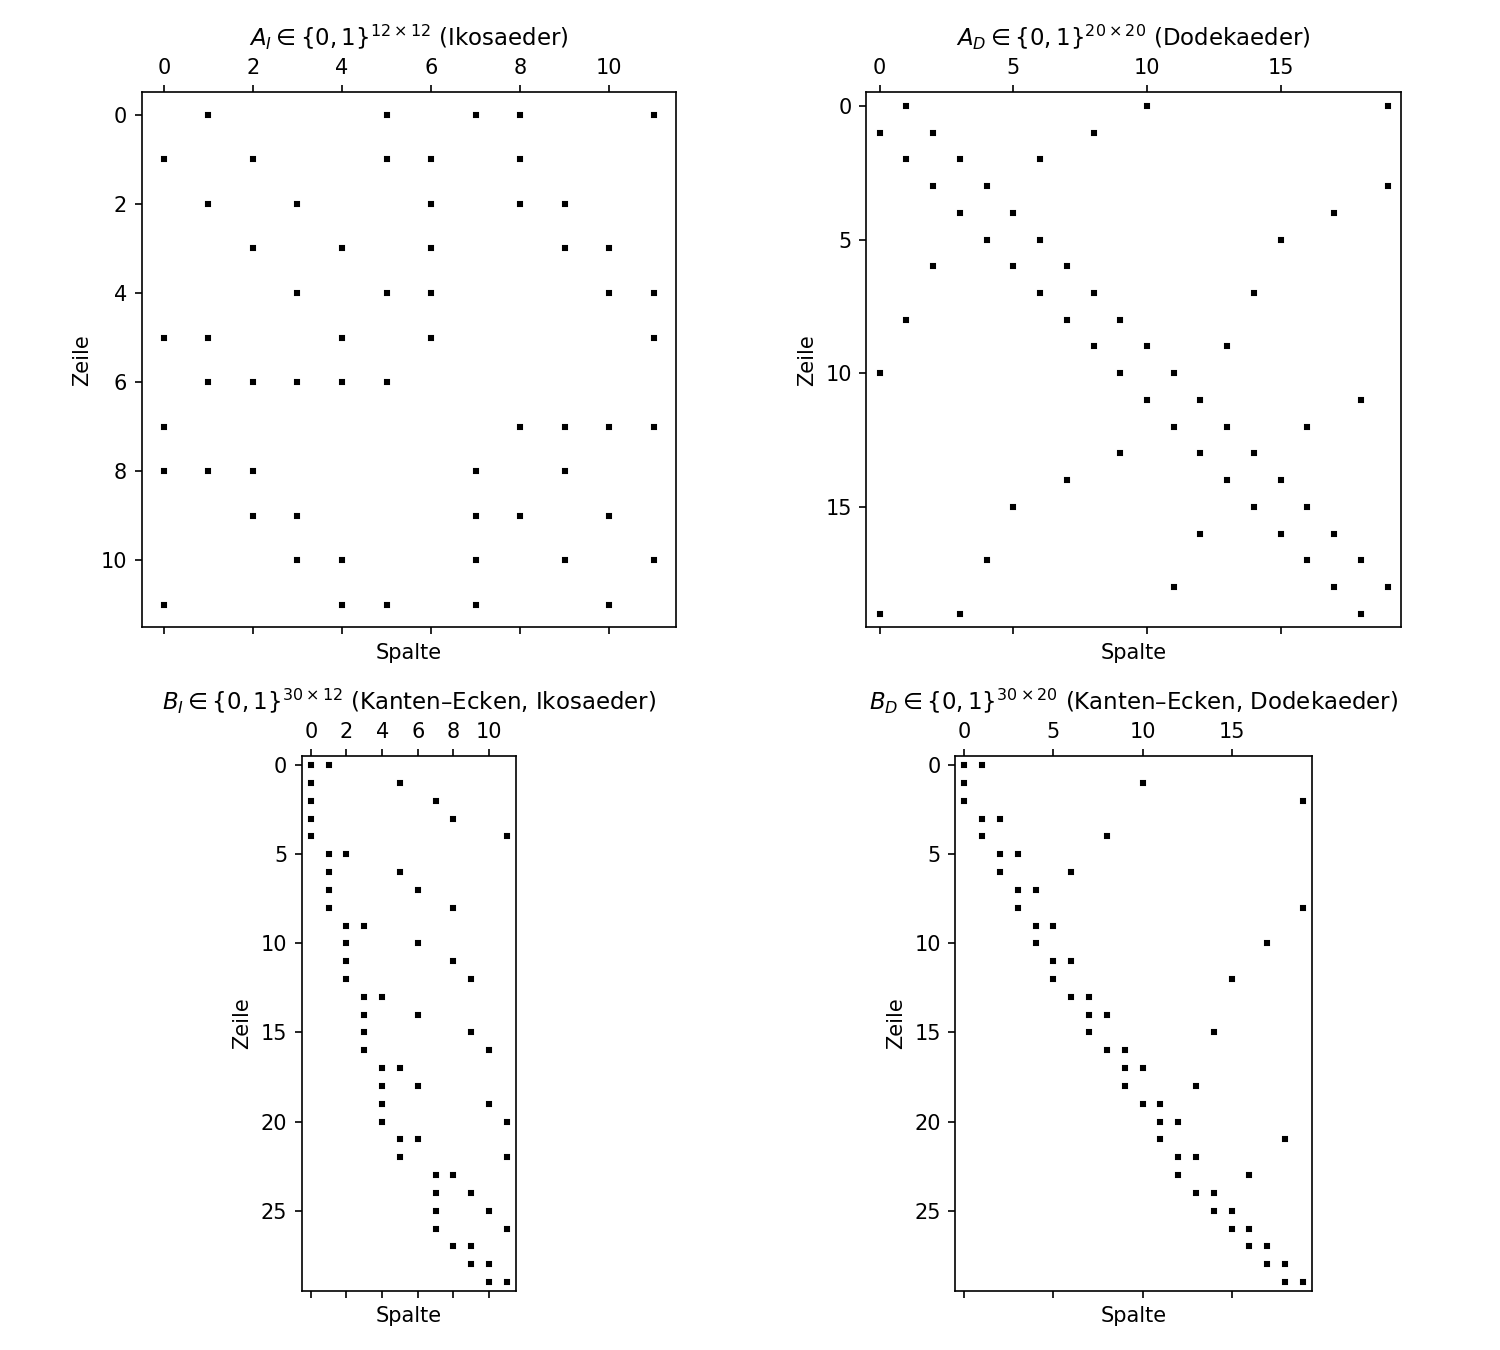
\includegraphics[width=0.92\linewidth]{ikodo_four_matrices.png}\\[0.8em]
  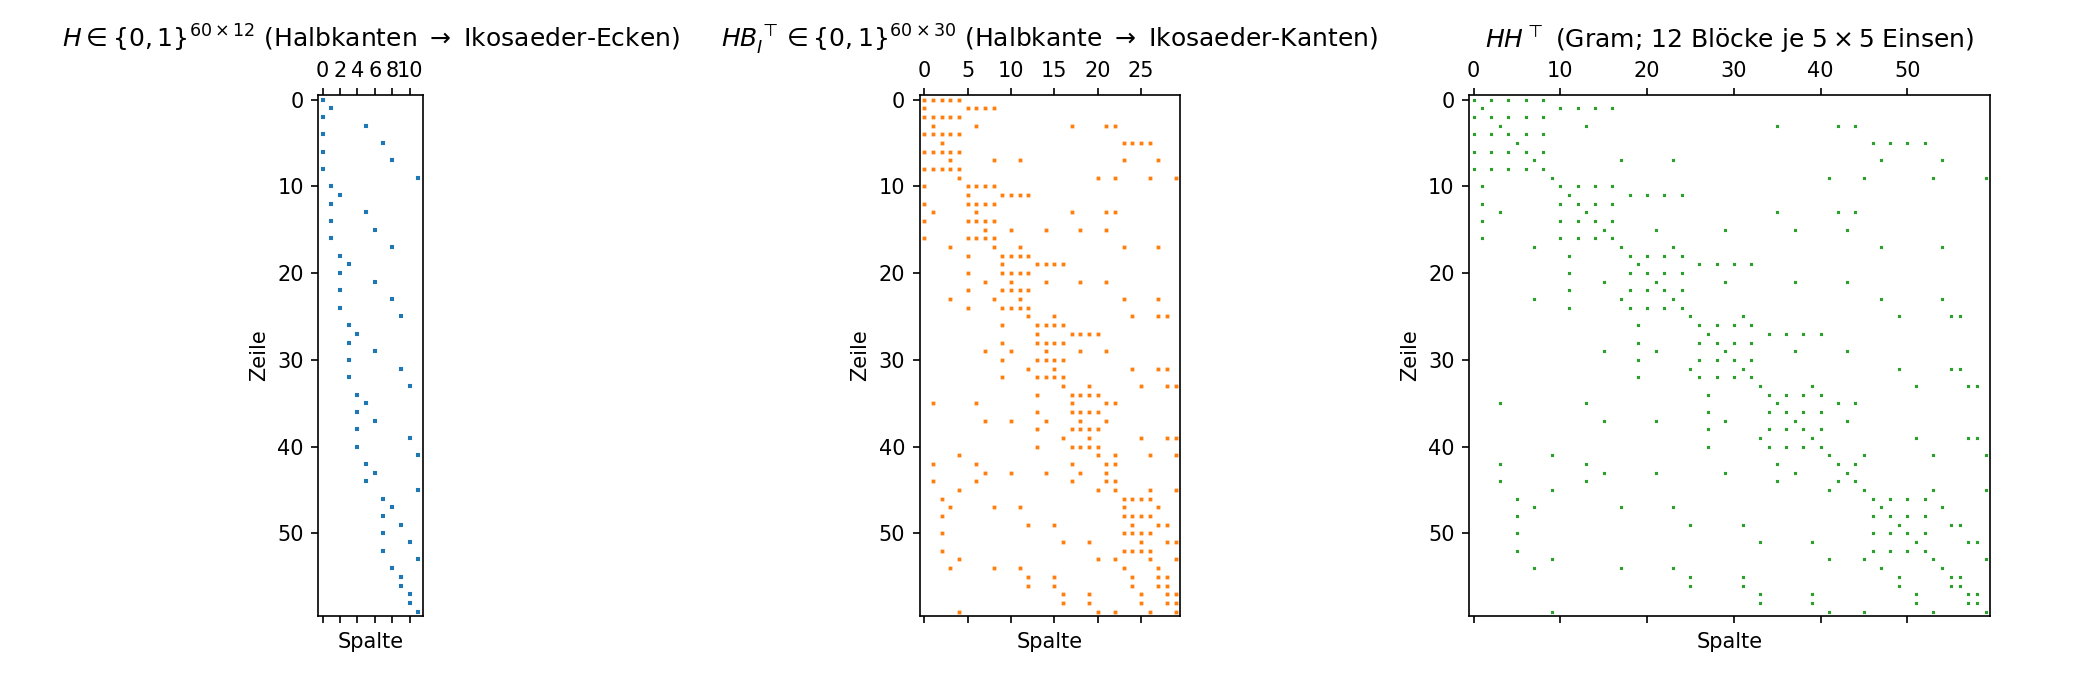
\includegraphics[width=\linewidth]{ikodo_transition_products.png}
  \caption{Oben: die vier Basismatrizen. Unten: Halbkanten-Matrix $H$, das Produkt
  $H B_I^{\mathsf T}$ und die Gram-Matrix $H H^{\mathsf T}$.}
\end{figure}

\end{document}
